%
% bewegung.tex -- Begründet die Bewegung von Wirbelringen
%
% !TEX root = ../../buch.tex
% !TEX encoding = UTF-8
%
\section{Bewegung \label{paper:Wirbelringe:Bewegung}}

Bisher wurde die Bewegung eines Wirbelrings noch nicht weiter betrachtet. 
Doch wie man bereits von Rauchringen beobachten kann, bewegen sich Wirbelringe. 
Betrachtet man zunächst ein Wirbelfaden, würde auffallen, dass sich dieser nicht bewegt. 
Daher, die Bewegung entsteht durch das Schliessen der Wirbellinie in einen Kreis. 
Um diese Verhalten begründen zu kann das Biot-Savart-Gesetz \cite{Wirbelringe:FuehrerdurchdieStroemungslehre} angewendet werden, welches im Folgenden formuliert werden soll.

\subsection{Biot-Savart-Gesetz}

Das Biot-Savart-Gesetz
\[
d \vec{B}
=
\frac{\mu_0}{4\pi}\frac{I \,d \vec{l} \times \vec{r}}{\left\lvert \vec{r}^{3}\right\rvert }
\]  % Note : diese Definition weicht von der Definiton 3.2 im ELT2 Skript ab da dort ein Richtungsvektor verwendet wird -> ein r (dort ein R) kürzt sich heraus
wird typischerweise in der Elektrotechnik angewendet, um das Magnetfeld von bewegten Ladungen zu beschreiben (hier nur auf einen Strom durch einen Leiter vereinfacht). 
Es kann nur bei geschlossenen Stromkreisen verwendet werden. 

Damit wir das Gesetz nutzen können, müssen wir zunächst die Grössen anpassen und überprüfen, ob das überhaupt erlaubt ist. 
Die elektrodynamischen Grössen haben jeweils ein Gegenstück in der Strömungsmechanik:

\begin{center}
    \begin{tabular}{lcl}
    stromdurchflossener Leiter          & \(\Leftrightarrow \) & Wirbelfaden \\
    Stromstärke \(I\)                   & \(\Leftrightarrow \) & Zirkulation \(\Gamma\) \\
    magnetische Feldstärke \(\vec{H}\)  & \(\Leftrightarrow \) & Geschwindigkeit \(\vec{u}\) \\
    \end{tabular}
\end{center}

Die Maxwellgleichungen (Siehe Abschnitt \ref{chapter:maxwell} ToDo : genaue Ref zu Maxwell) sehen auch vor das \(\vec{B}\) Feld quellenfrei ist. 
Da wir nur Inkompressible Fluide betrachten ist dies gegeben.

Setzt man nun die entsprechenden Grössen in das Biot-Savart-Gesetz ein 
\[
d \vec{v}
=
\frac{\Gamma}{4\pi}\frac{d \vec{l} \times \vec{r}}{\left\lvert \vec{r}^{3}\right\rvert }
\]
lässt sich damit die Geschwindigkeit eines Punktes in der Nähe eines Wirbelrings berechnen. 
Am einfachsten ist der Mittelpunkt des Kreises der Wirbellinie. 
Somit ist die Geschwindigkeit dieses Punktes
\[
\vec{v}
=
\int_{0}^{2\pi} \frac{\Gamma r}{4\pi}\frac{d \vec{l} \times \vec{r}}{\left\lvert \vec{r}^{3}\right\rvert },
\]
wobei \(r\) der Radius des Rings der Wirbellinie ist (und \(\Gamma\) die Zirkulation des Wirbelfadens). 
Da der Kreisumfang und der Radius immer senkrecht zueinander sind, folgt 
\[
\vec{v}
=
\frac{\Gamma r}{4\pi r^{3}} \int_{0}^{2\pi} \hat{z}\, dl,
\]
wobei \(\hat{z}\) in Ausbreitungsrichtung zeigt welche senkrecht auf Radius und Kreis steht. 
Schlussendlich ergibt sich
\[
\vec{v}
=
\frac{\Gamma }{2 r^2}\hat{z},
\]
woraus ersichtlich ist das, je kleiner der Wirbelring, desto schneller bewegt er sich.

Würde man das ganze für eine Gerade Wirbelröhre durchrechnen, würde auffallen, dass das Ergebnis null ist. 
Daher, damit sich eine Wirbelröhre von sich bewegt, muss sie zumindest ein wenig gekrümmt sein.

\subsection{Bewegung eines Teilchens}

\begin{figure}
\centering
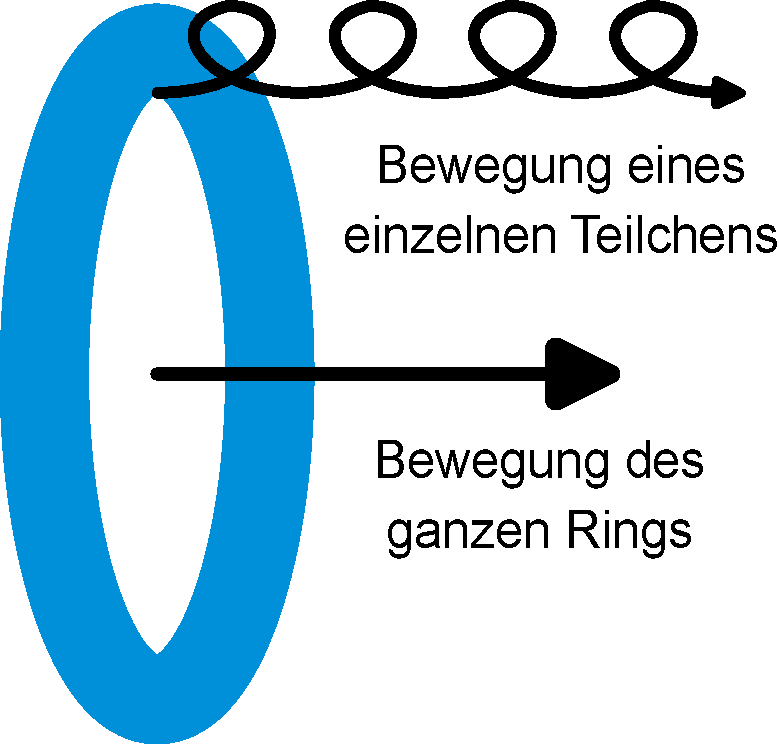
\includegraphics[width=0.4\textwidth]{papers/wirbelringe/fig/ausbreitung_teilchen.pdf}
\caption{Bewegung eines einzelnen Teilchen ToDo besseri Farb für de Ring??? \label{buch:papers:Wirbelringe:fig:ausbreitung_teilchen}}
\end{figure}

Eine interessante Kurve zeichnet sich ab, wenn man ein einzelnes Teilchen beobachtet. 
Es bildet sich eine verzogene Ellipse, welche untereinander verbunden ist. 
Die Grösse der Ellipse hängt von der Höhe der Zirkulation ab. 
Dies ist in Abbildung \ref{buch:papers:Wirbelringe:fig:ausbreitung_teilchen} dargestellt.
